\label{ch:results_and_sensitivity}

В данной главе представлены результаты вычислительных экспериментов по анализу чувствительности ресурсной системы массового обслуживания. Описываются выбранные параметры имитационной модели, сценарии изменения входящего потока и распределения времени обслуживания. Оценивается влияние распределения объёма работы заявки и типа входящего потока на вероятность отказа, пропускную способность, среднее число заявок в системе и средний занятый ресурс. Приводится интерпретация полученных результатов.

\section{Параметры вычислительного эксперимента}
\label{sec:exp_params}

Входные данные для имитации были подобраны таким образом, чтобы рассмотреть систему в различных состояниях\cite{jain1991_performance_analysis,law2015_simulation_modeling}; особый интерес представляют значения при которых система близка к критическим состояниям, так как здесь чувствительность проявляется наиболее четко\cite{jain1991_performance_analysis}. В текущей постановке задачи параметры системы зафиксированы следующим образом:  обслуживающие приборы $N = 96$, ограничение по ресурсу $R = 590$, скорость обслуживания $\mu = 1.2$ и интенсивность входящего потока $\lambda$, которая принимает значения $90, 104, 116$ для низкого среднего и высокого уровня нагрузки соответственно. 

Распределение случайного требования к ресурсу $D$ представлено в таблице~\ref{tab:resource_dist}.

\begin{table}[h!]
    \centering
    \caption{Распределение случайного требования к ресурсу $D$}
    \label{tab:resource_dist}
    \begin{tabular}{|l|c|c|c|c|c|}
        \hline
        \textbf{Значение ($d_i$)} & 2 & 4 & 8 & 12 & 16 \\ \hline
        \textbf{Вероятность ($p_i$)} & 0.25 & 0.25 & 0.30 & 0.15 & 0.05 \\ \hline
    \end{tabular}
\end{table}

Среднее требование к ресурсу для одной заявки, в соответствии с распределением в таблице~\ref{tab:resource_dist}, составляет $6.5$. При полной занятости обслуживающих устройств ($n=N$) суммарный требуемый ресурс составил бы $N \cdot \mathbb{E}[D] = 96 \cdot 6.5 = 624$ единицы, что превышает доступную емкость $R = 590$, поэтому отказов по ресурсу будет больше, что позволит лучше проиллюстрировать реальные системы, в которых зачастую также присутствует диспропорция\cite{naumov_total_resources_2016,naumov_samouylov_multiresource_loss_2017}. 

Время работы системы в ходе одной репликации задается дискретно-событийно и установлено на уровне $T_{max} = 50000$ условных единиц времени, из которых $T_{\text{warm}} = 5000$ --- время разогрева. При значениях интенсивности входящего потока $\lambda \in [90, 116]$, обеспечивается обработка от $3,5 \times 10^6 \text{ до } 5,8 \times 10^6$ заявок в рамках одной репликации. 

Для получения статистически достоверных оценок стационарных характеристик и подавления шума Монте-Карло, каждый сценарий моделировался серией из $R_{\text{rep}} = 40$ независимых репликаций с различными инициализирующими значениями генератора псевдослучайных чисел\cite{law2015_simulation_modeling,fishman1996_monte_carlo}. Согласно ЦПТ  $R_{\text{rep}} > 30$ достаточен для корректной аппроксимации целевых метрик нормальным законом и позволяет надежно рассчитывать $95\%$-ные доверительные интервалы. 

\section{Сценарии анализа чувствительности}
\label{sec:sensitivity_scenarios}

Для оценки чувствительности показателей эффективности системы (вероятности отказа в обслуживании) к некоторой комбинации распределения интенсивности входящего потока и времени работы были сформированы наборы случайных величин для интервалов поступления ($A$) и объемов работы ($W$), имеющие идентичные математические ожидания, но различные коэффициенты вариации $C_v$ (табл.~\ref{tab:dist_families}).

\begin{table}[h!]
    \centering
    \caption{Типы распределений для анализа чувствительности}
    \label{tab:dist_families}
    \begin{tabular}{|l|c|c|c|c|}
        \hline
        \textbf{Параметр} & \multicolumn{4}{c|}{\textbf{Варианты распределений}} \\ \hline
        Входящий поток (Arrival) & Poisson & $Erlang_2$ & $Erlang_4$ & $Hyperexp_2$ \\ \hline
        Время работы (Workload) & Deterministic & Exponential & $Erlang_4$ & Hyperexp \\ \hline
    \end{tabular}
\end{table}

\subsection{Компьютерное моделирование входящего потока}

Распределение входящего потока заявок определяет временную структуру нагрузки на систему. Выбранные семейства распределений для интервалов между поступлениями $A$:

\begin{enumerate}
    \item Пуассоновский поток, при котором интервалы времени между заявками распределены экспоненциально: $f(t) = \lambda e^{-\lambda t}$, где коэффициент вариации $C_v = 1$. Это базовое распределение входящего потока, обладающее марковостью, относительно которого в дальнейшем замеряются отклонения\cite{bocharov_pechinkin_tmo,adan_resing2015_queueing_systems}.
    \item Регулярные потоки Erlang-2 и Erlang-4, использующее распределение Эрланга $k$-го порядка\cite{adan_resing2015_queueing_systems}:
    $$
        f(t) = \frac{(k\lambda)^k t^{k-1} e^{-k\lambda t}}{(k-1)!}
    $$
    Для $Erlang_4$ коэффициент вариации $C_v = 0.5$. Эти сценарии моделируют входящий поток, где заявки поступают наиболее равномерно по сравнению с другими распределениями.
    \item Поток Hyperexp-2\cite{vishnevskii_dudin_correlated_arrivals_2017,paxson_floyd_1995_poisson_failure}. Моделируется как смесь двух экспоненциальных распределений с $C_v > 1$:
    $$
        f(t) = p \lambda_1 e^{-\lambda_1 t} + (1-p) \lambda_2 e^{-\lambda_2 t}.
    $$
    Выбор данного распределения обусловлен необходимостью анализа всплесков (burstiness), когда заявки приходят плотными группами за короткие промежутки времени, что часто провоцирует отказы системы.
\end{enumerate}

\subsection{Компьютерное моделирование времени обслуживания}

Выбор распределений для объема работы заявки $W$ позволяет оценить разные семейства распределения времени работы к ранее описанным входящим потокам. 

\begin{enumerate}
    \item Детерминированное обслуживание описывает сценарий, где $C_v = 0$, а $W = \mathbb{E}[W]$ постоянно; служит для оценки поведения системы в условиях идеальной предсказуемости обслуживания.
    \item Экспоненциальное обслуживание служит для проверки классических аналитических свойств системы.
    \item Erlang-4 имеет низкую вариативность и моделирует процессы обслуживания с устойчивым временем выполнения.
    \item Высоковариативное обслуживание с коэффициентом вариации ($C_v \gg 1$) и моделирует ситуацию, когда часть заявок обслуживается быстро, а отдельные занимают систему существенно дольше среднего. 
    В условиях ограниченного ресурса это распределение работы способно блокировать систему при стабильном потоке заявок; заявки периодически обслуживаются пачками.
\end{enumerate}

Параметры распределений во всех сценариях подобраны так, чтобы математическое ожидание соответствовало заданному уровню нагрузки: $\mathbb{E}[W] = 1/\mu = 0.833$.  

\section{Чувствительность к распределению объёма работы заявки}
\label{sec:workload_sensitivity_results}

Основная цель данного раздела заключается в проверке гипотезы о сохранении свойства инвариантности в РСМО, что подтверждается на полученных данных: переход от экспоненциального распределения к детерминированному, распределению Эрланга или гиперэкспоненциальному закону при сохранении идентичного среднего значения $\mathbb{E}[W] = 1/\mu$ не приводит к статистически значимым изменениям ключевых показателей эффективности\cite{sevastyanov1957_ergodic_refusals,burman1981_insensitivity,sopin2018_insensitivity}. 

На рисунке~\ref{fig:workload_main_metrics} представлены основные показатели системы в зависимости от интенсивности нагрузки для различных типов распределения обслуживания.

\begin{figure}[H]
    \centering
    
\includegraphics[width=0.95\textwidth]{workload_sensitivity_main_metrics_sigma-1p2}
    \caption{Основные показатели эффективности системы при различных распределениях времени обслуживания}
    \label{fig:workload_main_metrics}
\end{figure}

Анализ относительного смещения показателей относительно марковского экспоненциально распределенного базиса, представленные на рисунке~\ref{fig:workload_delta}, показывают, что девиации большинства метрик от не превышают долей процента.

\begin{figure}[H]
    \centering
    
\includegraphics[width=0.85\textwidth]{workload_sensitivity_delta_from_baseline_sigma-1p2}
    \caption{Относительное отклонение метрик от базового распределения обслуживания}
    \label{fig:workload_delta}
\end{figure}

Эффект от изменения формы распределения времени обслуживания сопоставим с уровнем статистического шума метода Монте-Карло, как видно из диаграммами размаха на рисунке~\ref{fig:workload_boxplot}. Средние значения находятся практически на одной линии. 

\begin{figure}[H]
    \centering
    
\includegraphics[width=0.85\textwidth]{workload_sensitivity_boxplot_loss_probability_sigma-1p2_lambda-116}
    \caption{Диаграмма размаха вероятности потери для различных типов обслуживания ($\lambda = 116$)}
    \label{fig:workload_boxplot}
\end{figure}

При этом межквартильные размахи (ширина «ящиков»), отражающие дисперсию результатов между независимыми репликациями, полностью перекрывают друг друга.

На рисунке~\ref{fig:workload_stationary} показана оценка стационарного распределения числа заявок в системе $\pi(k)$.

\begin{figure}[H]
    \centering
    
\includegraphics[width=0.95\textwidth]{workload_sensitivity_stationary_distribution_sigma-1p2_lambda-116}
    \caption{Оценка стационарного распределения вероятностей состояний $\pi(k)$ ($\lambda = 116$)}
    \label{fig:workload_stationary}
\end{figure}

Кривые вероятностей состояний для детерминированного, экспоненциального, эрланговского и гиперэкспоненциального законов обслуживания совпадают на всем диапазоне возможных состояний.

\subsection*{Выводы по разделу}
При марковском (пуассоновском) входящем потоке в исследуемой ресурсной системе чувствительность к закону распределения времени работы заявки практически отсутствует. Все зафиксированные расхождения не превышают долей процента и полностью объясняются дисперсией метода Монте-Карло. Полученный результат согласуется с классическим свойством инвариантности  стационарного распределения\cite{sevastyanov1957_ergodic_refusals,burman1981_insensitivity,sopin2018_insensitivity}. 

Таким образом, для данного режима работы подтверждена возможность использования простейших экспоненциальных аппроксимаций $M/M/N/R$ без потери точности моделирования \cite{dudin2025_random_environment}.
% Главная идея раздела:
% workload сам по себе почти не меняет стационарные характеристики,
% особенно при пуассоновском входе.
%
% Это не слабый результат, а важный результат:
% он показывает, что модель ведёт себя согласно известной инвариантности.
%
% Здесь лучше не писать "результатов нет".
% Писать надо так:
% "наблюдается слабая чувствительность", "эффект сопоставим с шумом Монте-Карло",
% "результат согласуется с инвариантностью".

\section{Чувствительность к типу входящего потока}
\label{sec:arrival_sensitivity_results}

В данном разделе анализируется влияние типа входящего потока на показатели эффективности ресурсной системы с потерями\cite{paxson_floyd_1995_poisson_failure,leland_taqqu_willinger_wilson_1994_selfsimilar,vishnevskii_dudin_correlated_arrivals_2017}. Рассматриваются следующие типы входящего потока$\{\text{Poisson}, \text{Erlang-2}, \text{Erlang-4}, \text{HyperExp-2}\}$, при фиксированном детерминированном распределении времени работы.

Во всех сценариях данного раздела выполняется условие $\mathbb{E}[A] = \frac{1}{\lambda},$
где $A$ --- случайный межприходный интервал. Базовым сценарием для сравнения выбран пуассоновский поток $a_0 = \text{Poisson}$.

На рисунке~\ref{fig:arrival_main_metrics} представлены основные показатели эффективности системы при различных типах входящего потока и уровнях интенсивности $\lambda$.

\begin{figure}[H]
    \centering
    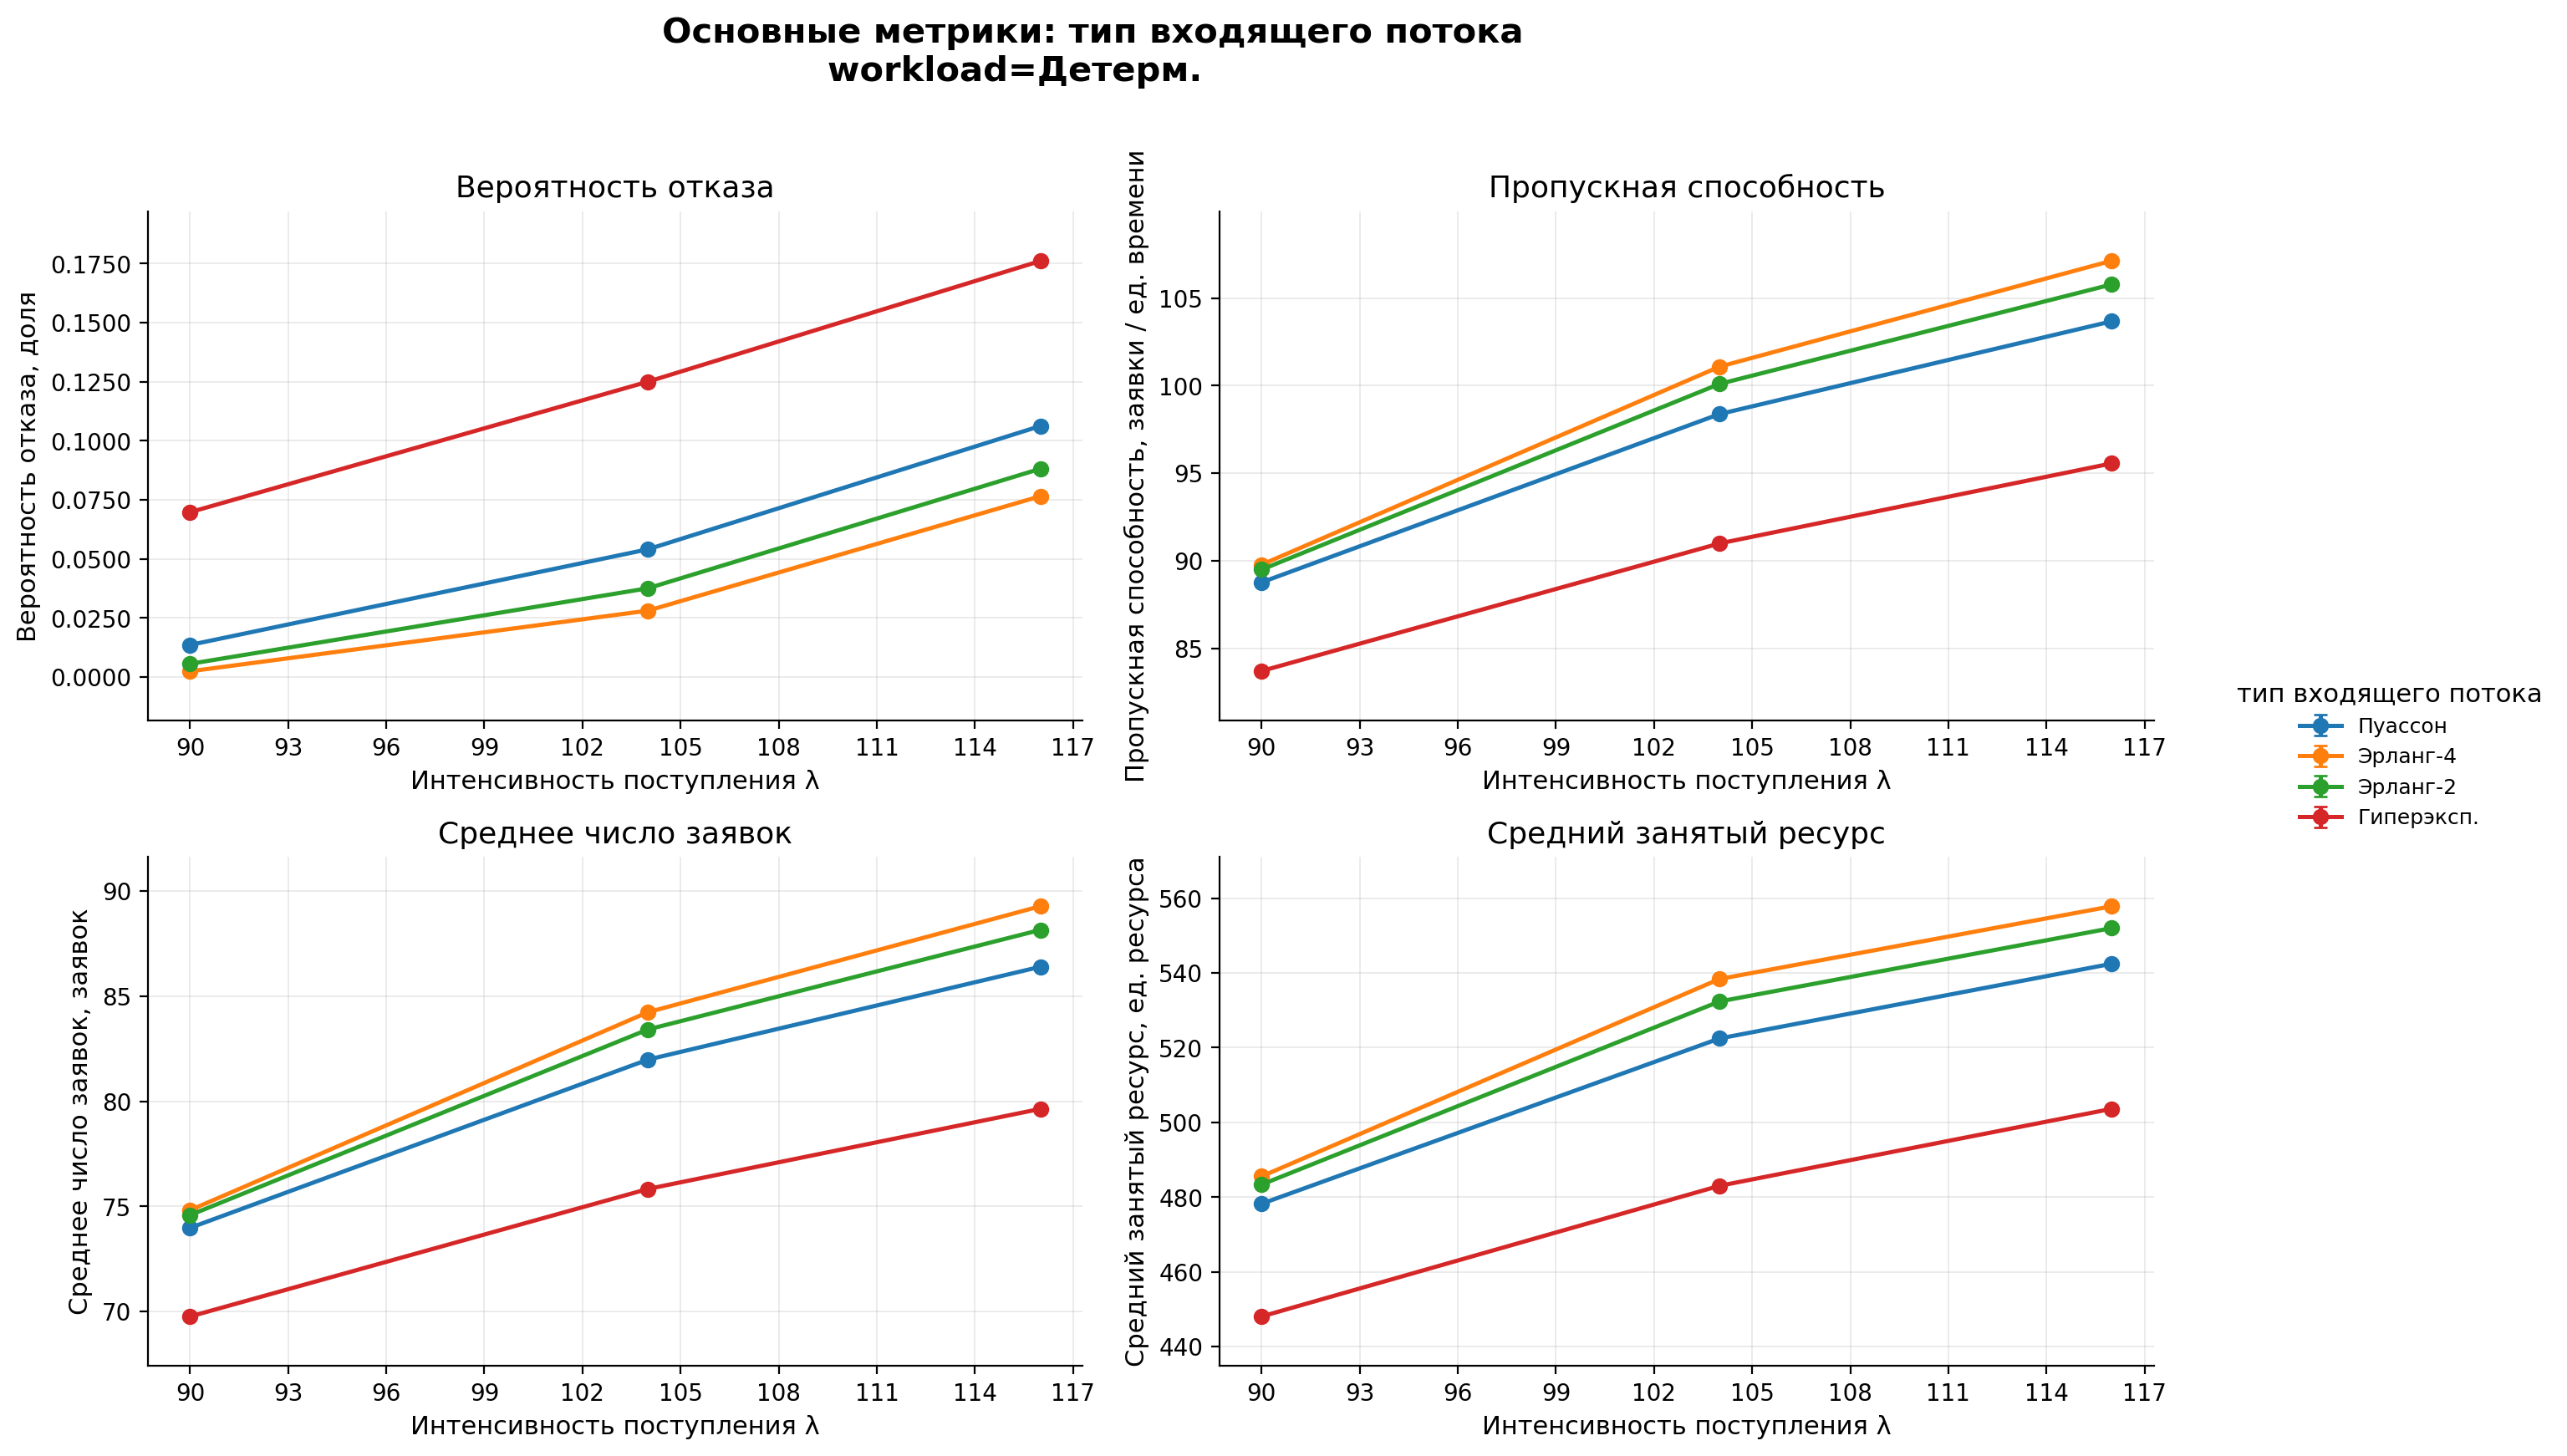
\includegraphics[width=0.95\textwidth]{images/arrival_sensitivity_main_metrics_sigma-1p2.png}
    \caption{Основные показатели эффективности системы при различных типах входящего потока}
    \label{fig:arrival_main_metrics}
\end{figure}

При увеличении $\lambda$ вероятность отказа возрастает; темп роста различается для разных распределений. Наименьшие значения вероятности отказа наблюдаются для регулярных эрланговских потоков, а наибольшие --- для гиперэкспоненциального потока.


На рисунке~\ref{fig:arrival_loss_bars} отдельно показана вероятность отказа по уровням интенсивности $\lambda$.

\begin{figure}[H]
    \centering
    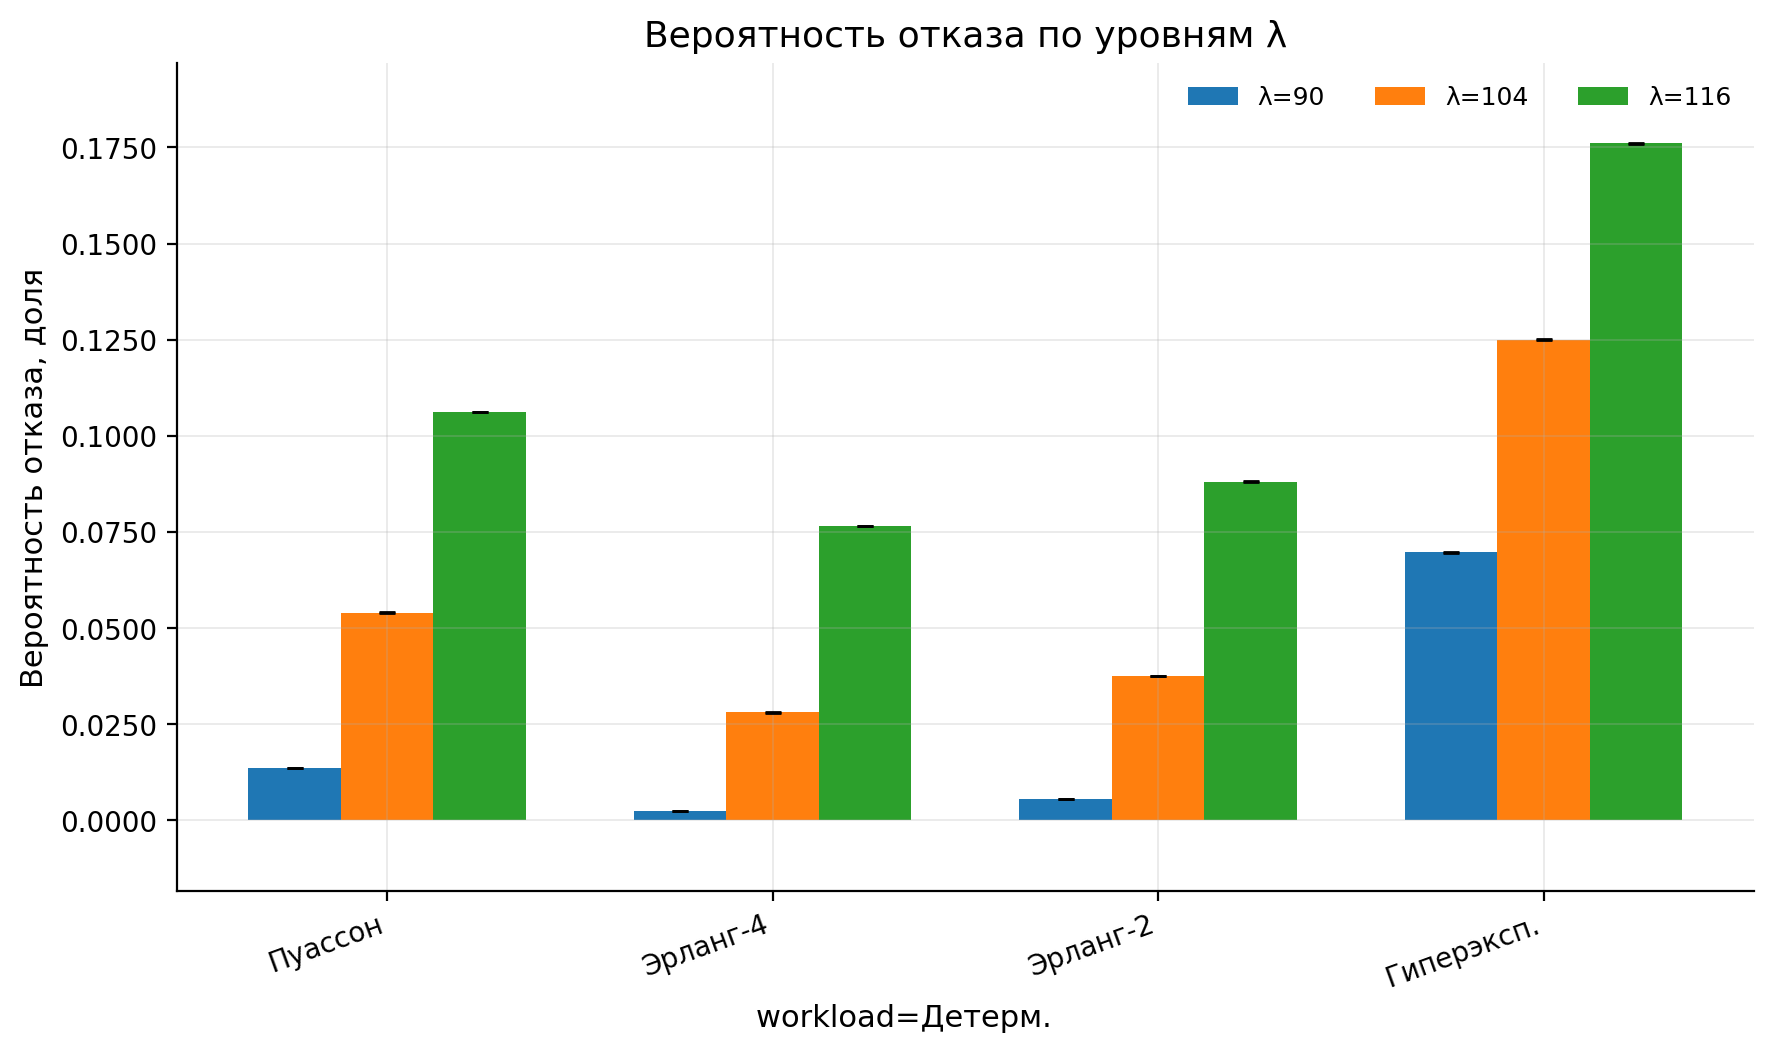
\includegraphics[width=0.90\textwidth]{images/arrival_sensitivity_loss_probability_bars_by_lambda_sigma-1p2.png}
    \caption{Вероятность отказа при различных типах входящего потока и уровнях $\lambda$}
    \label{fig:arrival_loss_bars}
\end{figure}

Чем больше $\lambda$ тем более выраженным становится различие между различными распределениями входящего потока. Гиперэкспоненциальный поток даёт максимальную вероятность отказа, а поток Эрланга четвёртого порядка остаётся наиболее благоприятным.


Для проверки устойчивости полученных различий были построены диаграммы размаха по независимым репликациям\cite{tukey1977_exploratory_data_analysis}. Ниже приведён разброс вероятности отказа при $\lambda=116$.

\begin{figure}[H]
    \centering
    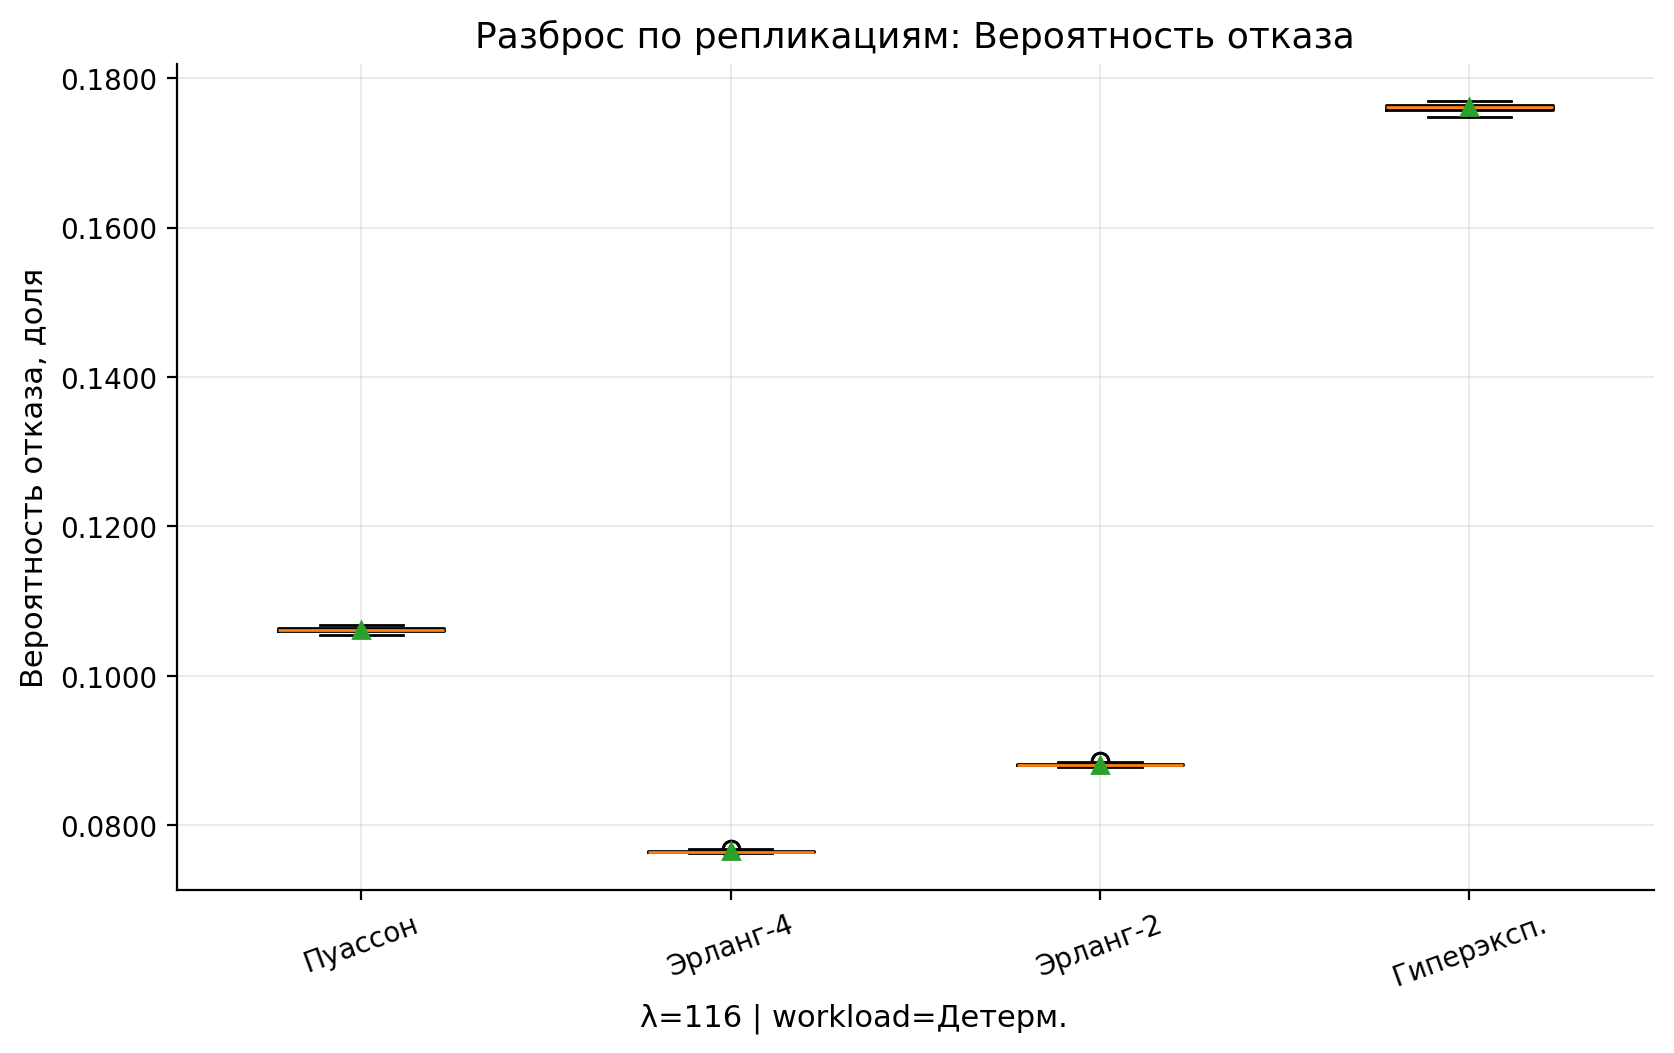
\includegraphics[width=0.90\textwidth]{images/arrival_sensitivity_boxplot_loss_probability_sigma-1p2_lambda-116.png}
    \caption{Разброс вероятности отказа по репликациям при $\lambda=116$}
    \label{fig:arrival_boxplot_loss}
\end{figure}

Видно, что межсценарные различия значительно превышают внутрисценарный разброс по репликациям. Наблюдаемая чувствительность к типу входящего потока не является следствием шума Монте-Карло\cite{law2015_simulation_modeling,welch1983_statistical_analysis_simulation}. В отличие от результатов по распределению workload, здесь различия между сценариями статистически выражены.

На рисунке~\ref{fig:arrival_stationary_dist} показано исследование $\pi(k)$ при $\lambda = 116$.

\begin{figure}[H]
    \centering
    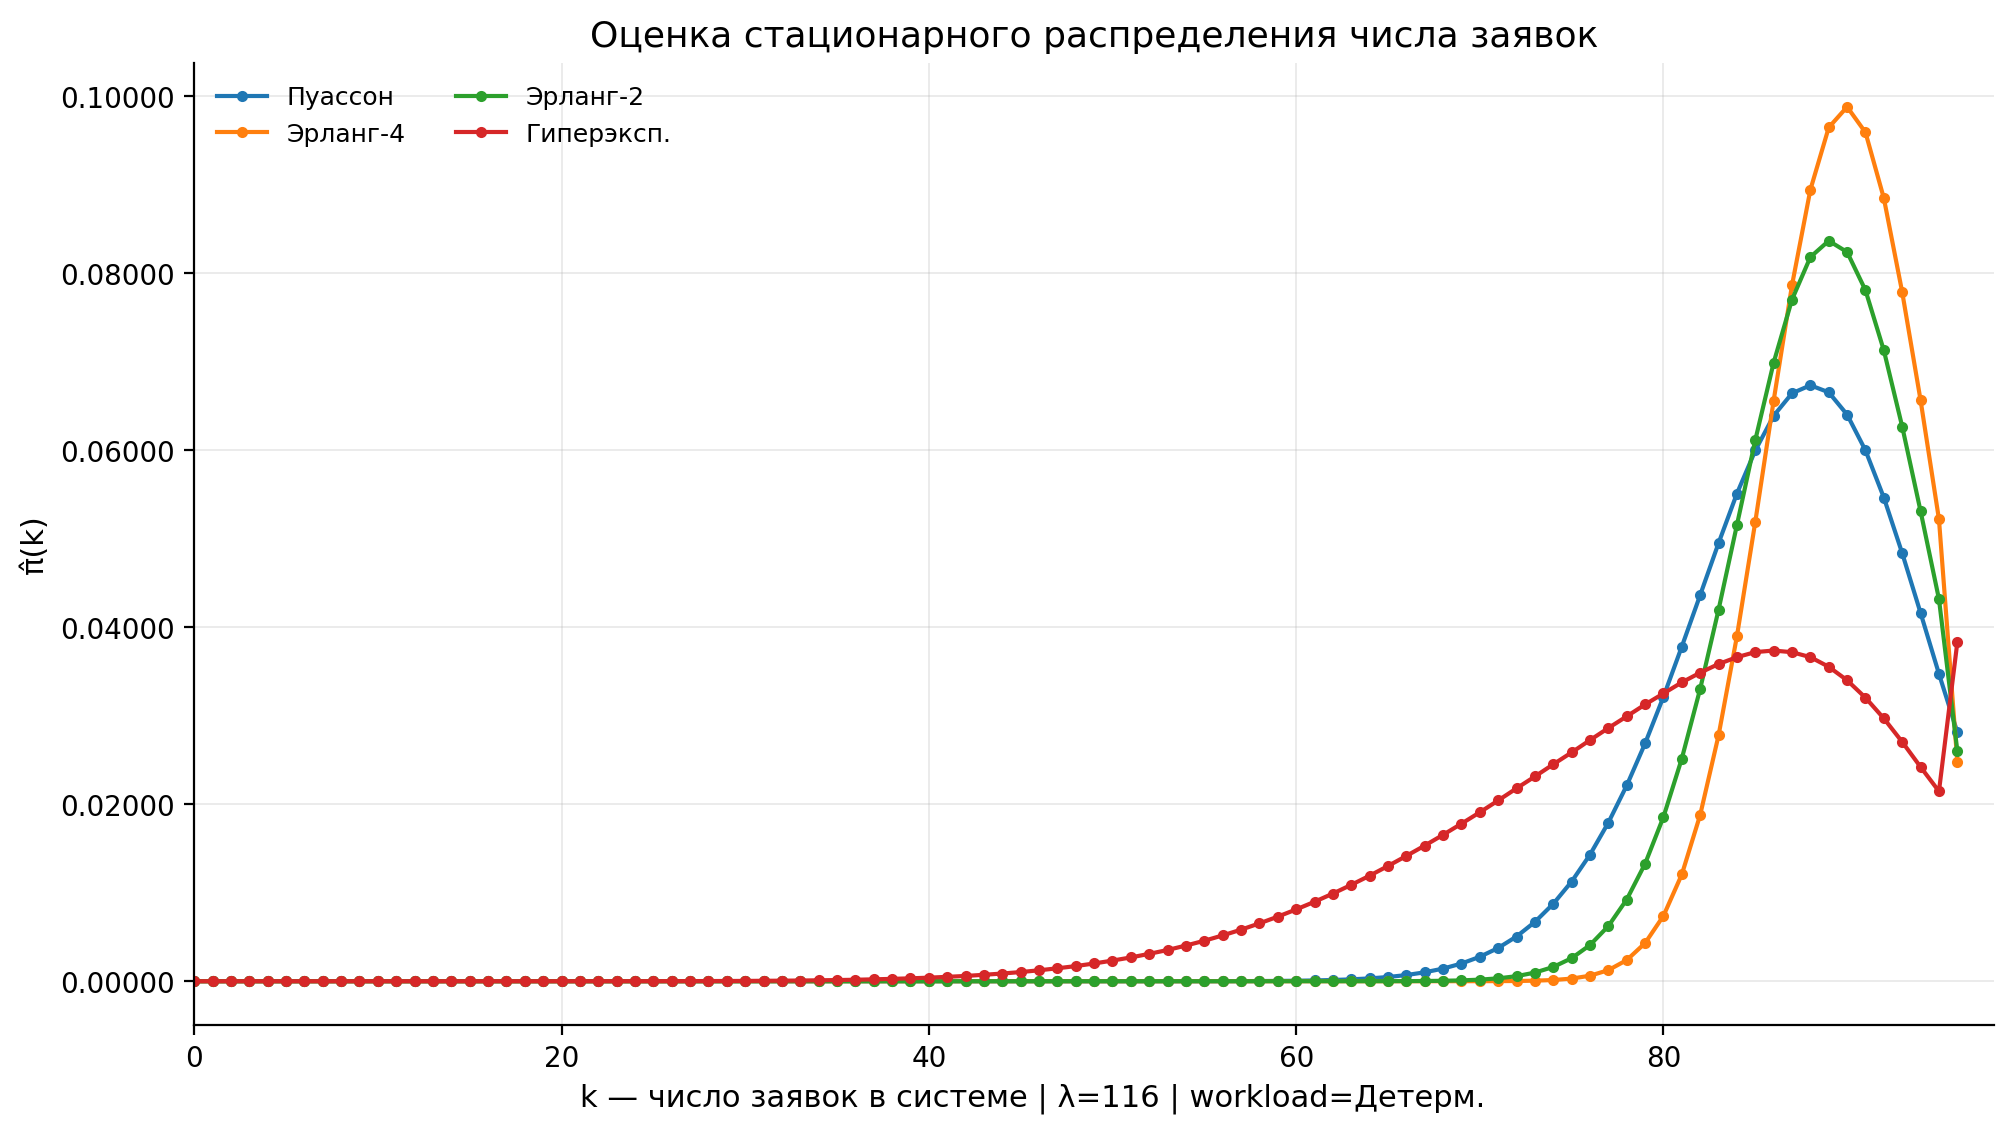
\includegraphics[width=0.95\textwidth]{images/arrival_sensitivity_stationary_distribution_sigma-1p2_lambda-116.png}
    \caption{Стационарное распределение числа заявок в системе $\pi(k)$ при различных типах входящего потока ($\lambda = 116$)}
    \label{fig:arrival_stationary_dist}
\end{figure}

Кривые на графике сильно варьируются, для регулярных потоков распределение смещено в сторону больших значений $k$. При гиперэкспоненциальном входящем потоке распределение $\pi(k)$ более пологое, но растет ближе к левому краю из-за редких приходов больших пачек заявок.

Дополнительно была построена оценка хвоста стационарного распределения числа заявок в системе~\ref{fig:arrival_stationary_tail}.

\begin{figure}[H]
    \centering
    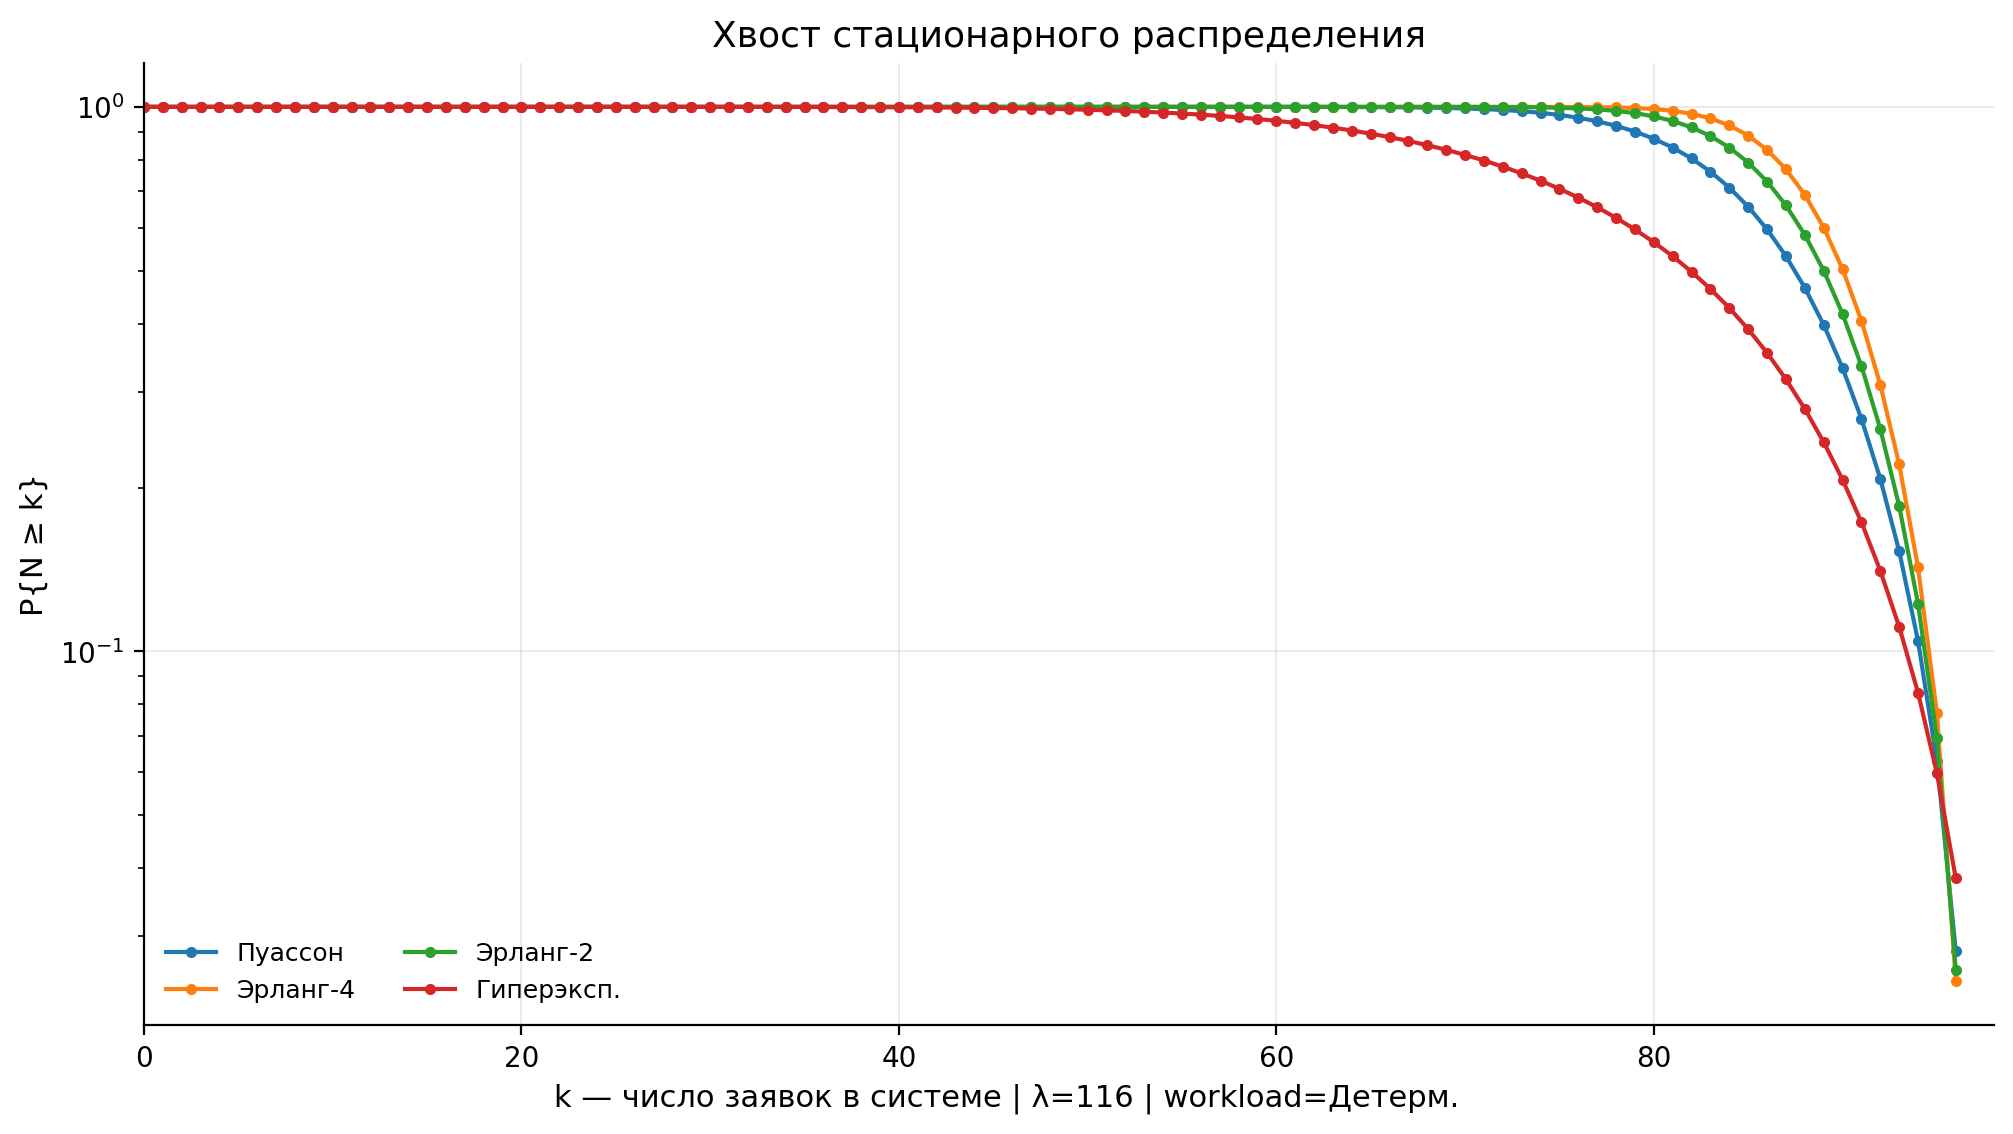
\includegraphics[width=0.95\textwidth]{images/arrival_sensitivity_stationary_tail_sigma-1p2_lambda-116.png}
    \caption{Хвост стационарного распределения числа заявок в системе при $\lambda=116$}
    \label{fig:arrival_stationary_tail}
\end{figure}

Хвостовое распределение подтверждает различие режимов заполнения системы. Для регулярных эрланговских потоков распределение держится на высоких (много заявок в системе) устойчивых значениях - загрузка равномерная. У гиперэкспоненциального входящего потока хвост убывает медленнее - высокая вероятность состояний с высокой занятостью системы, множество отказов по ресурсу $R$.

\subsection*{Выводы по разделу}

Тип входящего потока является ключевым факторов чувствительности ресурсной системы с потерями\cite{paxson_floyd_1995_poisson_failure,vishnevskii_dudin_correlated_arrivals_2017}. При одинаковом $\lambda$ различные распределения межприходных интервалов приводят к принципиально разной вероятности отказа, пропускной способности и средней занятости.

Регулярные потоки Эрланга уменьшают вероятность отказа, а гиперэкспоненциальный поток увеличивает вероятность отказа из-за локальных перегрузок. 

% Главная идея:
% Это основной результат главы.
% При одинаковой средней интенсивности lambda разные распределения межприходных интервалов
% дают заметно разные p_loss, throughput, mean_num_jobs и mean_occupied_resource.
%
% Особенно важно:
% Erlang-потоки более регулярные, HyperExp-поток более bursty.
% Поэтому сравнение идет не по среднему, а по вариативности межприходных интервалов.

\section{Совместное влияние распределения обслуживания и входного потока}
\label{sec:combined_sensitivity_results}

В данном разделе анализируется полный набор сценариев, в котором одновременно варьируются тип входящего потока $a$, распределение объёма работы заявки $\omega$ и интенсивность поступления $\lambda$.

Каждый сценарий можно записать в виде
$$
s = (a, \omega, \lambda, \mu, N, R, F_D),
$$
где $a$ --- тип входящего потока, $\omega$ --- тип распределения workload, $\lambda$ --- средняя интенсивность поступления, $\mu$ --- скорость обслуживания, $N$ --- число обслуживающих каналов, $R$ --- общий объём ресурса, $F_D$ --- распределение ресурсного требования заявки. 

В рамках проводимых экспериментов зафиксированы $N = 96, R = 590, \mu = 1.2, F_D$ заданы таблично, следовательно каждый экспериментальный сценарий однозначно задается сокращенным вектором $s' = (a, \omega, \lambda)$. Базовым сценарием является детерминированный workload и пуассоновский входящим потоком $
s'_0(\lambda) = (\text{Poisson}, \text{Deterministic}, \lambda)$.

Взаимное влияние этих переменных на показатели системы удобно отражать в тепловых картах, так, например,  на рисунке ~\ref{fig:combined_loss_matrix} показана веротяность отказа.

\begin{figure}[H]
    \centering
    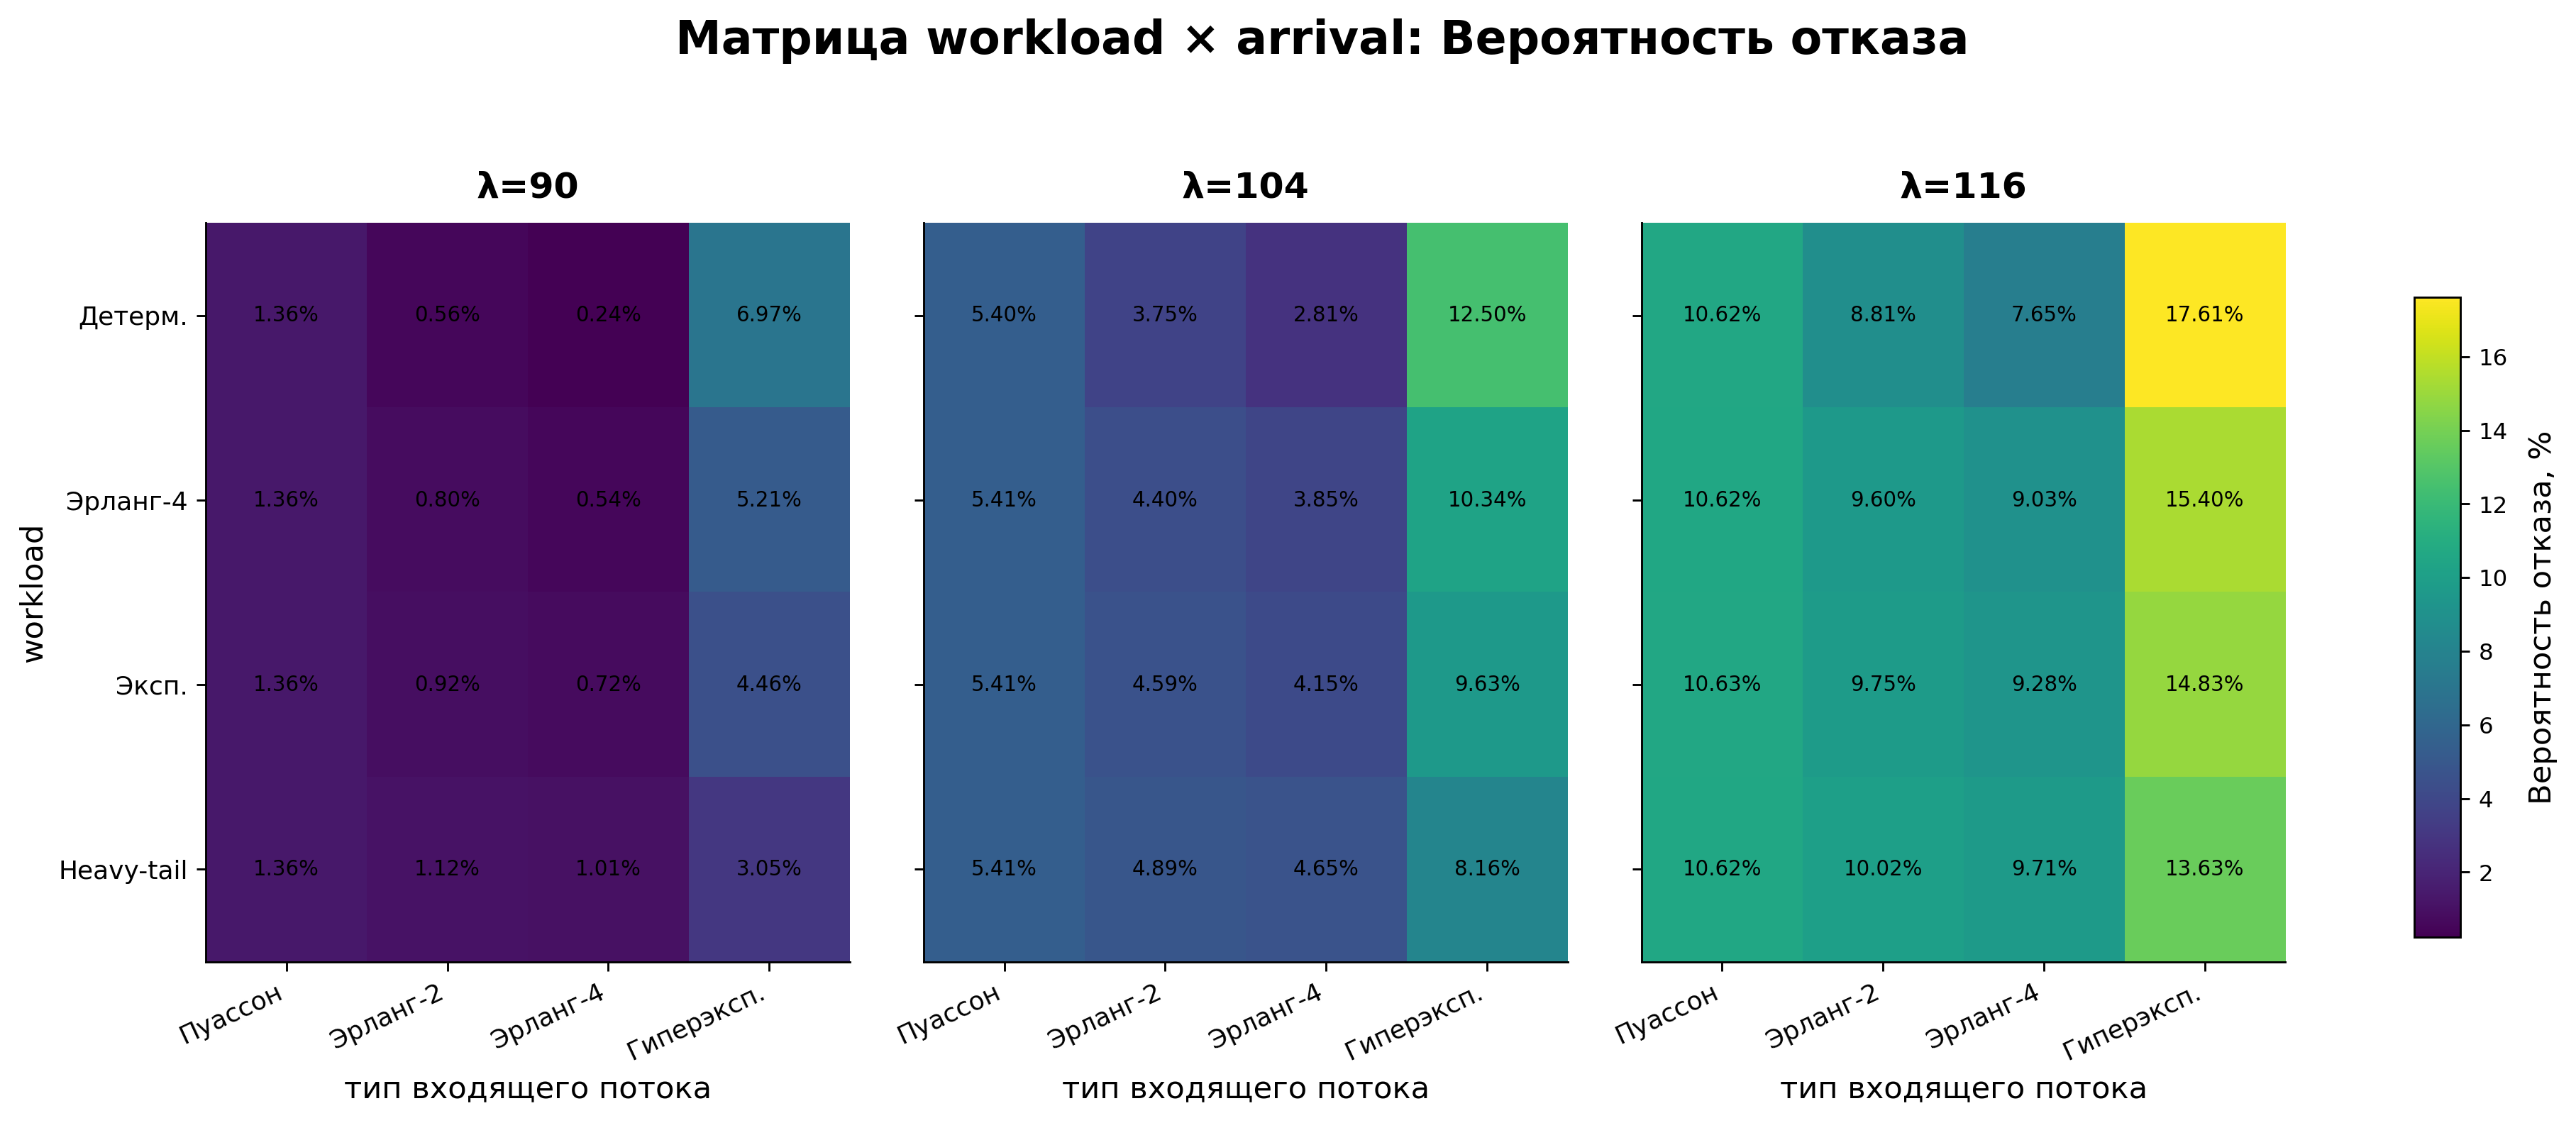
\includegraphics[width=0.98\textwidth]{images/01_heatmap_workload_arrival_loss_probability_sigma-1p2.png}
    \caption{Матрица workload $\times$ arrival для вероятности отказа}
    \label{fig:combined_loss_matrix}
\end{figure}


% !!!Переменные без крышки - теоретические значения. Переменные с крышкой - эмпирическая оценка.
% m - просто метрика

При пуассоновском входящем потоке $P_{\text{loss}}$ практически не зависит от распределения workload, как было ранее установлено в ~\ref{sec:workload_sensitivity_results}. При $c_A^2 = 1$, изменение $c_B^2$ практически не меняет вероятность отказа. Например, при $\lambda=116$ для всех четырёх workload расхождения вероятности отказа находятся на уровне $0.01$ процентного пункта: $10.62\%,\quad 10.62\%,\quad 10.63\%,\quad 10.62\%$. 
Это подтверждает инвариантность РСМО относительно распределения времени обслуживания при пуассоновском входе.

При непуассоновских входящих потоках инвариантность по распределению workload нарушается\cite{paxson_floyd_1995_poisson_failure,vishnevskii_dudin_correlated_arrivals_2017}, причём знак эффекта зависит от вариативности входящего потока. Для регулярных потоков Эрланга увеличение вариативности workload повышает вероятность отказа, а для гиперэкспоненциального входа, наоборот, снижает её; выполняется следующий порядок квадратов коэффициентов вариации:
$$
c_A^2(\text{Erlang-4}) < c_A^2(\text{Erlang-2}) < c_A^2(\text{Poisson}) < c_A^2(\text{HyperExp}),
$$
где
$$
\begin{aligned}
    c_A^2(\text{Erlang-4}) &= 0.25, & c_A^2(\text{Erlang-2}) &= 0.5, \\
    c_A^2(\text{Poisson}) &= 1, & c_A^2(\text{HyperExp}) &> 1.
\end{aligned}
$$

Для регулярных входящих потоков наблюдается наименьшая вероятность отказа, но чем выше вариативность workload, тем больше будет вероятность отказа. При $\lambda=116$ и входящем потоке Erlang-4 значения вероятности отказа соответствуют следующим workload:
$$
\begin{aligned}
    \text{Deterministic} = 7.65\% \rightarrow \text{Erlang-4} = 9.03\% \\
    \rightarrow \text{Exponential} = 9.28\% \rightarrow \text{Heavy-tail} = 9.71\%,
\end{aligned}    
$$
Для Erlang-2:
$$
8.81\% \rightarrow 9.60\% \rightarrow 9.75\% \rightarrow 10.02\%,
$$
Абсолютный рост между детерминированным и heavy-tail workload составляет 2.06 процентного пункта для Erlang-4 и 1.21 для Erlang-2. Следовательно, для регулярного входа выполняется соотношение $\frac{\partial P_{\mathrm{loss}}}{\partial c_B^2} > 0$. Регулярный поток лучше всего сочетается с регулярным обслуживанием.

Для гиперэкспоненциального входящего потока знак эффекта меняется. При $\lambda=116$ вероятность отказа уменьшается при росте вариативности workload, выполняется обратная зависимость:
$$
17.61\% \rightarrow 15.40\% \rightarrow 14.83\% \rightarrow 13.63\%.
$$
Выполняется обратная зависимость $\frac{\partial P_{\mathrm{loss}}}{\partial c_B^2} < 0$, так как гиперэкспоненциальный поток создаёт пачки поступлений и детерменированный workload долго выходит из перегрузок, а более вариативные режимы освобождают ресурс пачечно и снижают отказ. 

Поведение остальных метрик согласуется с формулой пропускной способности: $\theta = \lambda(1 - P_{\mathrm{loss}})$. При фиксированной $\lambda$ рост вероятности отказа автоматически снижает throughput. Поэтому сценарии с Erlang arrival имеют большую пропускную способность, а сценарии с HyperExp arrival --- меньшую. Разница между Erlang-4 и HyperExp при $\lambda = 116$ составляет $107.1 - 95.6 = 11.5$ заявки на единицу времени или почти на 11\%. Средний занятый ресурс ведёт себя аналогично.

% 3. Тепловая карта: Пропускная способность
\begin{figure}[H]
    \centering
    
\includegraphics[width=0.95\textwidth]{01_heatmap_workload_arrival_throughput_sigma-1p2}
    \caption{Тепловая карта пропускной способности системы при совместном варьировании распределений}
    \label{fig:comb_heatmap_throughput}
\end{figure}
% 2. Тепловая карта: Средний занятый ресурс
\begin{figure}[H]
    \centering
    
\includegraphics[width=0.95\textwidth]{01_heatmap_workload_arrival_mean_occupied_resource_sigma-1p2}
    \caption{Тепловая карта среднего занятого ресурса при совместном варьировании распределений}
    \label{fig:comb_heatmap_resource}
\end{figure}

Для вероятности отказа совместное смещение относительно базового сценария измеряется в процентных пунктах:
$$
\Delta p_{\mathrm{loss}}(a,\omega,\lambda)
=
100 \cdot
\left(
\widehat{p}_{\mathrm{loss}}(a,\omega,\lambda)
-
\widehat{p}_{\mathrm{loss}}(\text{Poisson},\text{Deterministic},\lambda)
\right).
$$

Для остальных метрик используется относительное отклонение:
$$
\delta_m(a,\omega,\lambda)
=
100 \cdot
\left(
\frac{\widehat{m}(a,\omega,\lambda)}
{\widehat{m}(\text{Poisson},\text{Deterministic},\lambda)}
-
1
\right).
$$

То есть на графиках сравниваются именно отклонения от базового сценария при той же самой интенсивности $\lambda$. Например, на рисунке~\ref{fig:comb_delta_arrival} представлена смещение arrival относительно пуассоновского входа при фиксированном workload.

\begin{figure}[H]
    \centering
    
\includegraphics[width=0.95\textwidth]{04_delta_arrival_vs_poisson_by_workload_loss_probability_sigma-1p2}
    \caption{Относительное отклонение вероятности потери от пуассоновского базлайна при различных распределениях обслуживания}
    \label{fig:comb_delta_arrival}
\end{figure}

Для Erlang-потоков $\Delta_A P_{\mathrm{loss}} < 0$, для гиперэкспоненциального входа $\Delta_A P_{\mathrm{loss}} > 0$. При $\lambda=116$ и детерминированном workload, где регуляризация входящего потока снижает вероятность отказа на $1.8\text{-}3.0$ п.п., а bursty-вход увеличивает её почти на $7$ п.п.: $\Delta_A P_{\mathrm{loss}}(\text{Erlang-2,Erlang-4, HyperExp}) = -1.809, -2.970, +6.986$ соответственно.

Распределение workload само по себе не имеет универсального положительного или отрицательного влияния, его эффект определяется типом входящего потока.
% 5. Дельта: Влияние workload при фиксированном arrival (vs Deterministic)
\begin{figure}[H]
    \centering
    
\includegraphics[width=0.95\textwidth]{05_delta_workload_vs_deterministic_by_arrival_loss_probability_sigma-1p2}
    \caption{Относительное отклонение вероятности потери от детерминированного обслуживания при различных входящих потоках}
    \label{fig:comb_delta_workload}
\end{figure}

Структура отказов подтверждает, что главным ограничением в рассматриваемой постановке является ресурс $R$, а затем только число серверов $N$. 
% 7. Структура отказов (Rejection breakdown)
\begin{figure}[H]
    \centering
    
\includegraphics[width=0.95\textwidth]{08_rejection_components_heatmaps_sigma-1p2}
    \caption{Структура отказов (доля блокировок по серверам и по ресурсу) при совместном варьировании распределений}
    \label{fig:comb_rejection_components}
\end{figure}
Менее равномерный вход увеличивает оба типа отказов, но основной вклад даёт именно ограничение по ресурсу. 

\subsection*{Выводы по разделу}

Совместный эксперимент показывает, что чувствительность РСМО с потерями связана с типом входящего потока. При одинаковом $\lambda$ регулярные Erlang-потоки уменьшают вероятность отказа, а гиперэкспоненциальный поток существенно увеличивает её. Сгладить влияние bursty потоков позволяет менее однородное распределение времени работы. 
 Для рассмотренных уровней нагрузки сохраняется порядок:
$$
P_{\mathrm{loss}}(\text{Erlang-4})
<
P_{\mathrm{loss}}(\text{Erlang-2})
<
P_{\mathrm{loss}}(\text{Poisson})
<
P_{\mathrm{loss}}(\text{HyperExp})
$$

Для РСМО с потерями необходимо учитывать прежде всего среднюю нагрузку, затем форму входящего потока и наконец её взаимодействие с распределением времени обслуживания.

% Главная идея:
% Отдельно workload почти слабый фактор.
% Но при непуассоновском входе он взаимодействует с arrival.
% Поэтому полезно ввести interaction effect.

\section{Практическая интерпретация результатов и выводы}
\label{sec:practical_interpretation}

% Главная идея:
% Здесь надо не повторить все графики, а собрать смысл.
%
% Структура:
% 1) что является главным фактором чувствительности;
% 2) где наблюдается инвариантность;
% 3) почему средняя lambda недостаточна;
% 4) что означает структура отказов;
% 5) что ограничивает выводы.

Вычислительные эксперименты проводились для РСМО с потерями $GI/G/N/N/R$ при фиксированных параметрах $N=96$, $R=590$, $\mu=1.2$, $\mathbb{E}[W]=1/\mu=0.833$. Интенсивность входящего потока принимала значения $\lambda \in \{90,104,116\}$. Распределение ресурсного требования $D$ задавалось значениями $2,4,8,12,16$ с вероятностями $0.25,0.25,0.30,0.15,0.05$, поэтому $\mathbb{E}[D]=6.5$. Каждый сценарий оценивался по $40$ независимым репликациям.

Основным фактором чувствительности в рассматриваемой системе является тип входящего потока. Различные распределения $A$ приводят к разнообразным значениям вероятности отказа, пропускной способности и средней занятости ресурса. Регулярные потоки Эрланга уменьшают вероятность отказа, а гиперэкспоненциальный поток, моделирующий всплески поступлений, существенно её увеличивает.

Вторым по значению фактором чувствительности является средняя интенсивность потока $\lambda$. 

Распределение объёма работы заявки $W$ при пуассоновском входящем потоке подтверждает свойство инвариантности системы. При непуассоновском входе инвариантность нарушается. Распределение времени обслуживания зависит от входящего потока заявок и может улучшить отказоустойчивость: при равномерном входящем потоке выигрыш дает равномерное распределение workload, при крайне неравномерном входящем потоке burstly workload позволяет снизить потери. Лучшим сочетанием является Erlang-4 входящий поток и deterministic workload, худшим гиперэкспоненциальный входящий поток и deterministic workload.

Декомпозиция отказов показывает, что в выбранной конфигурации главным ограничивающим фактором является ресурс $R$.
